\chapter{Path Plananing}\label{chap:Planning}

\section{Usage of the RRT* Vertices}

Chapter \ref{sec:trajectory} illustrates the optimization of a trajectory which passes through predefined vertices. From now on, the vertices are no longer chosen manually but are defined by the result of the RRT* algorithm. The computational efficiency of the RRT* algorithm combined with the positive features of the nonlinear optimization discussed in section \ref{sec:nonlinearopt} will lead to a optimized trajectory in densely packed environment.

\subsection{Vertex Extension}


Since the RRT* algorithm does not consider the dynamical behavior of a UAV there are still some challenges converting the RRT* straight line solution into a polynomial trajectory. In other words, there is the possibility that the polynomial trajectory passing through the vertices of the collision-free straight line solution is in collision with an obstacle. In this case a vertex, which is located on the straight line, has to be added. \newline

The process of generating a collision-free optimized trajectory can be summarized in following steps:


\begin{enumerate}
  \item Generate a collision-free straight line solution using the RRT* algorithm
  \item Create an initial trajectory passing through the vertices of the straight line solution
  \item If the initial solution is in collision, extend the existing vertices by a vertex located on the straight line solution. Compute the initial solution including the new vertex. Repeat this step until the trajectory is collision-free
\item Perform a nonlinear optimization on the collision-free trajectory
\item If the optimized solution is in collision, extend the existing vertices by a vertex located on the straight line solution and restart the nonlinear optimization. Repeat this step until the optimized trajectory is collision-free
\end{enumerate}

This schematic description of the process is depicted step by step in the subsequent figures for a better understanding.

\subsubsection{1. Generate a collision-free straight line solution using the RRT* algorithm}

Figure \ref{pic:RRTstepOne} depicts the straight line solution of the RRT* algorithm, which is explained in section \ref{sec:RRTstar}.  The $\gamma$ parameter, which is needed to calculate the radius $r$ in equation \ref{equ:ballradius}, is set to $\gamma = 1.5$. Furthermore, the edge length of the bounding box is set to $0.5m$ for each dimension. Although the hight of a UAV is commonly smaller than the length and the width this is required if great roll and pitch angles are permitted. \newline


Please note that, due to the randomness of the RRT* algorithm, the straight line solution depicted in figure  \ref{pic:RRTstepOne} is different than the straight line solution depicted in figure \ref{pic:bbx} even though the parameters are the same. 

\begin{figure}[h]
   \centering
   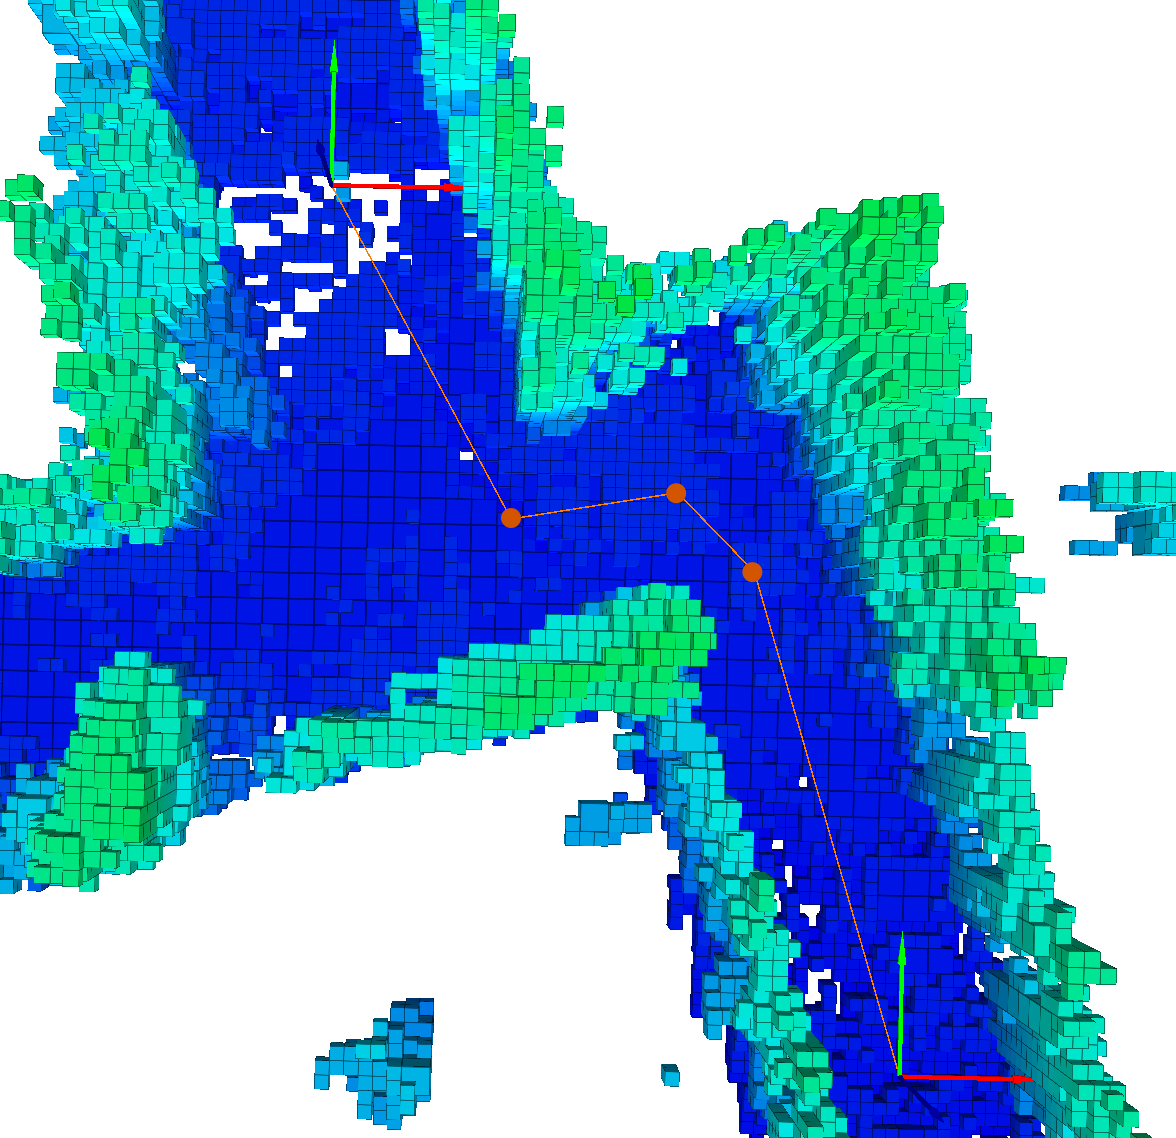
\includegraphics[trim = 45mm 0mm 35mm 0mm,clip,width=0.8\textwidth]{pics/extensionLongP.png}
   \caption{A collision-free straight line solution with 4 segments.}
   \label{pic:RRTstepOne}
\end{figure}


\subsubsection{2. Create an initial trajectory passing through the vertices of the straight line solution}

The start and goal vertex (each marked by a red and green arrow in figure \ref{pic:RRTstepOne}) as well ass the 3 vertices (each marked by a orange dot in figure \ref{pic:RRTstepOne}) defined by the solution of the RRT* algorithm are now used to generate the initial polynomial solution according to equation \ref{equ:dpstar} and equation \ref{equ:segmentTime}. \newline

The initial trajectory passing through the vertices of the RRT* algorithm is depicted in figure \ref{pic:RRTstepTwo}. The start vertex is in the upper left corner and the goal vertex is in the lower right corner. In the second segment there is a collision between the trajectory and the wall of the hallway (represented by green boxes). 

\begin{figure}[h]
   \centering
   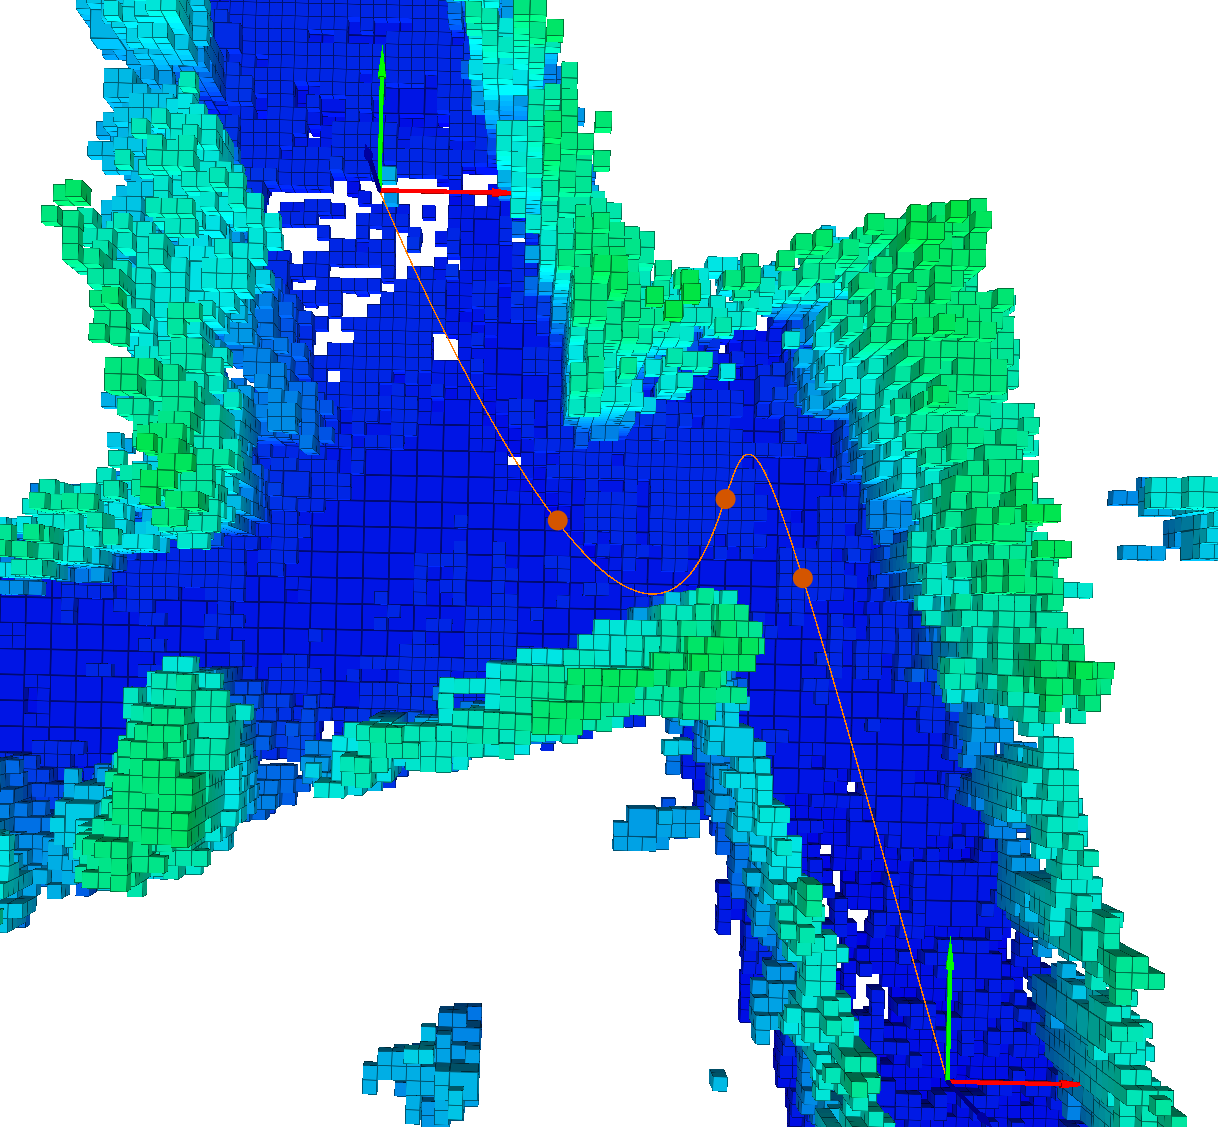
\includegraphics[trim = 45mm 0mm 35mm 0mm,clip,width=0.8\textwidth]{pics/extensionALongP.png}
   \caption{Initial trajectory with 4 segments. The start vertex is located in the upper left corner and the goal vertex is located in the lower right corner. There is a collision in the second segment of the trajectory.}
\label{pic:RRTstepTwo}
\end{figure}

\subsubsection{3. If the initial solution is in collision, extend the existing vertices by a vertex located on the straight line solution. Compute the initial solution including the new vertex. Repeat this step until the trajectory is collision-free}

To avoid the collision, a new vertex which is located on the straight line connection of the second segment has to be added. As a result, the trajectory is forced to stay closer to the straight line solution which is collision-free. \newline

The trajectory after one cycle of vertex extension is depicted in figure \ref{pic:RRTstep3}. A new vertex, represented by a red dot, is placed on the straight line connection of the second segment. \newline
As can be seen in figure \ref{pic:RRTstep3} the new vertex is not placed in the middle of the straight line connection. Especially if the segment is long and the collision is close to the start or the end of the segment, placing the new vertex in the middle is not an appropriate approach. \newline

\begin{figure}[h]
   \centering
   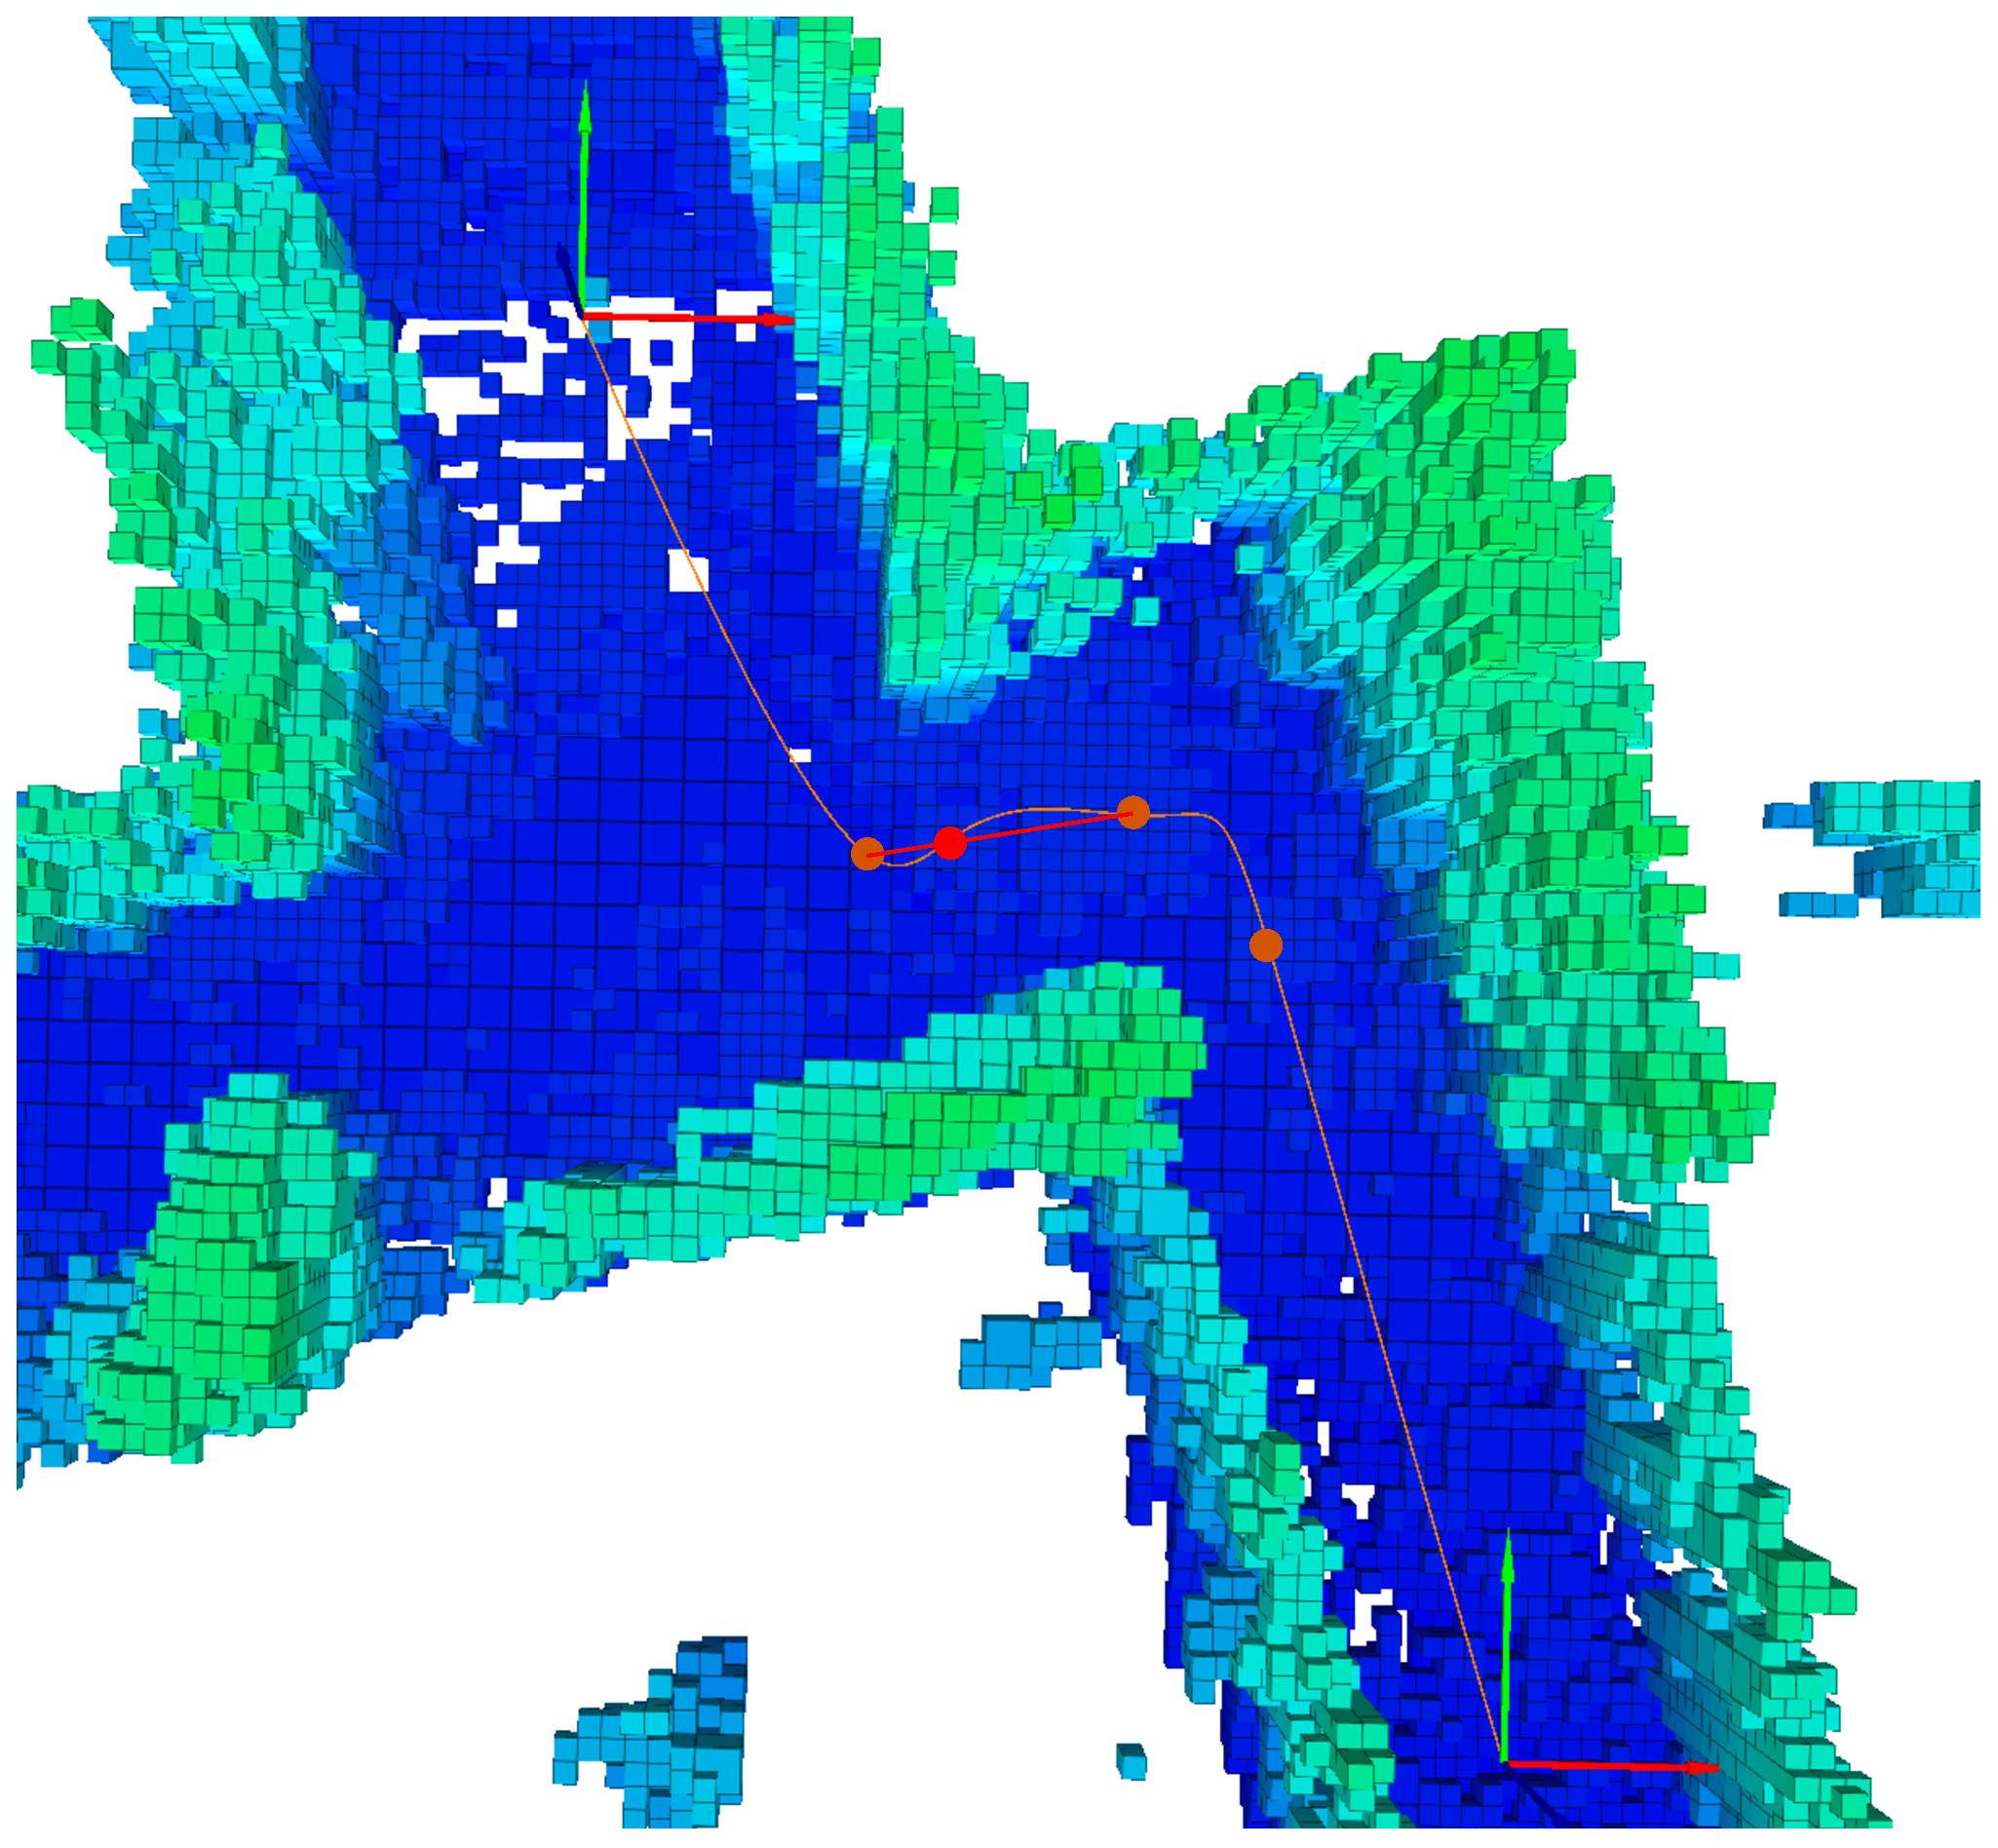
\includegraphics[trim = 45mm 0mm 35mm 5mm, clip,width=0.8\textwidth]{pics/extensionBLongPred.eps}
   \caption{Polynomial trajectory after a vertex extension, whereas the new vertex is represented by a red dot. The red line is not part of the trajectory but depicts the straight line connection of this segment.}
\label{pic:RRTstep3}
\end{figure}


To get an idea in which part of the trajectory the collision takes place, the length of the trajectory from the start of the segment to the collision is compared to the total trajectory length in this segment. This ratio is then mapped to the straight line solution and the additional vertex is placed. 
As explained in section \ref{sec:bbx}, the trajectory is in collision as soon as there is any obstacle inside the bounding box. Applied to the trajectory in figure \ref{pic:RRTstepTwo} this means that the collision is detected in the first half of the second segment before the trajectory itself proceeds through the wall of the hallway. Hence, the new vertex in figure \ref{pic:RRTstep3} is closer to the start of the second segment than to the end.



%\begin{figure}[h]
%   \centering
%   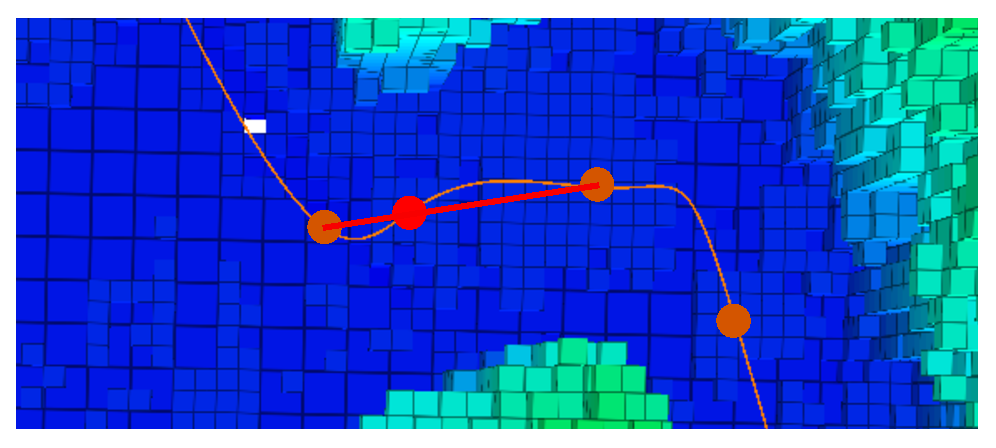
\includegraphics[width=1\textwidth]{pics/extensionBLongPredline.eps}
%   \caption{Ein Bild.}
%\end{figure}



\subsubsection{4. Perform a nonlinear optimization on the collision-free trajectory}

Using the trajectory depicted in figure \ref{pic:RRTstep3} as initial values a nonlinear optimization is performed. The optimized trajectory is depicted in figure \ref{pic:RRTstep4}. \newline


As mentioned in section \ref{sec:pathway}, the pathway of a snap minimized trajectory is mainly determined by the ratio of the segment times. Since the the ratio of the segment times of the trajectory in figure \ref{pic:RRTstep3} is not optimal the pathway contains unnecessary detours. \newline
After the nonlinear optimization, which includes an implicit optimization of the ratio of the segment times, the pathway is smoother and more suitable for a dynamic UAV flight.


\begin{figure}[h]
   \centering
   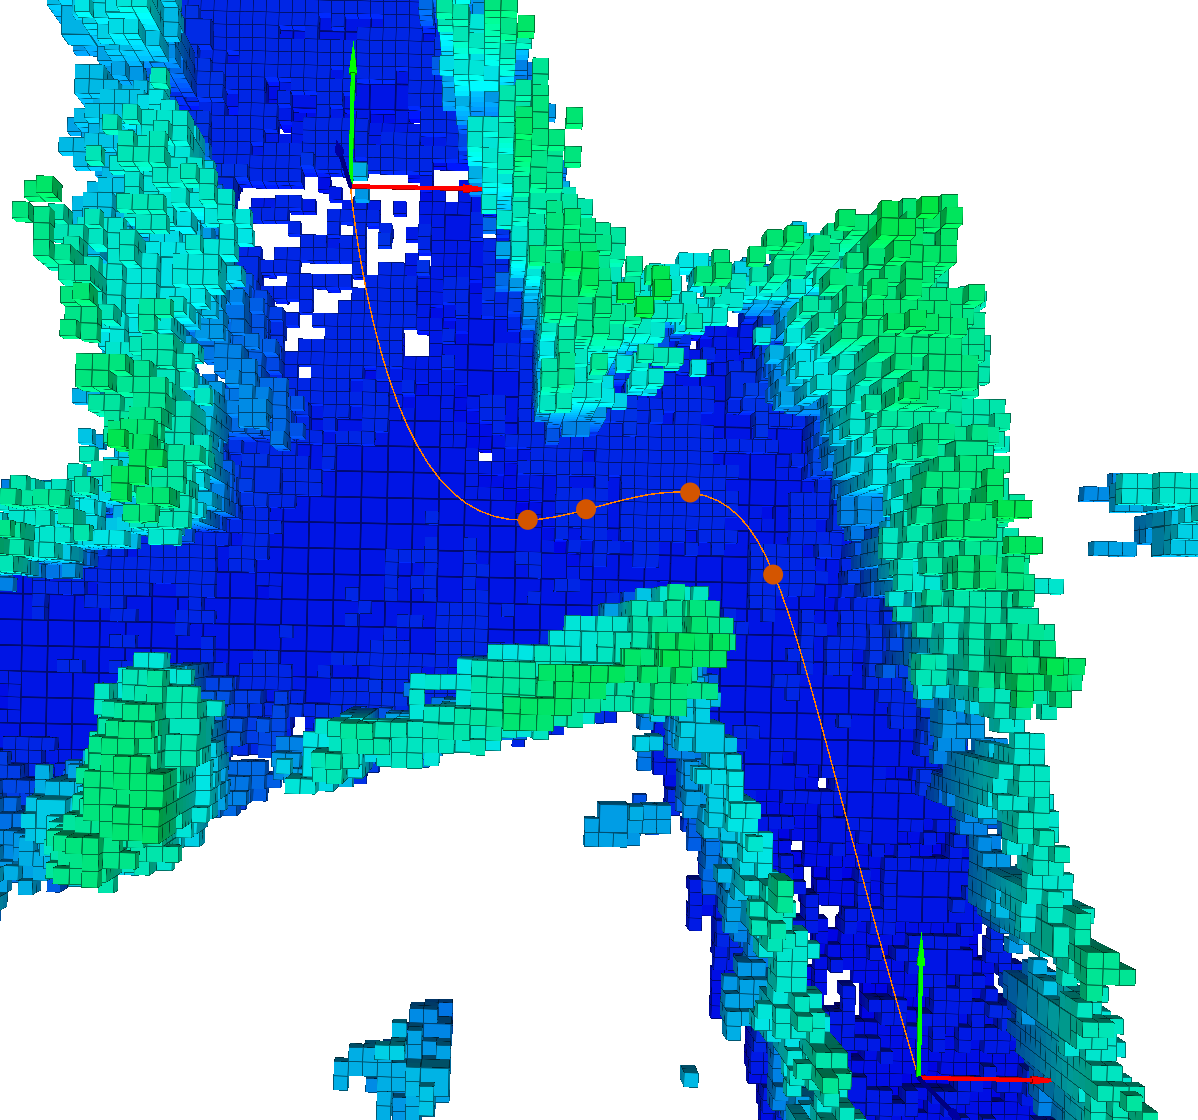
\includegraphics[trim = 60mm 0mm 35mm 0mm, clip,width=0.8\textwidth]{pics/extensionCLongP.png}
   \caption{The optimized trajectory with 5 segments.}
\label{pic:RRTstep4}
\end{figure}

\subsubsection{5. If the optimized solution is in collision, extend the existing vertices by a vertex located on the straight line solution and restart the nonlinear optimization. Repeat this step until the optimized trajectory is collision-free}
In this example the optimized trajectory is collision free without any further vertex extensions. Since the optimization smooths the trajectory but does not change the pathway of the trajectory completely, this is the general case. \newline

Nevertheless, if the optimized trajectory is in collision the vertex extension is equivalent to the procedure depicted in figure \ref{pic:RRTstep3}.

\subsection{Enlargement of the Bounding Box}\label{sec:enlargementBBX}

The initial trajectory passing through the vertices of the RRT* solution can be in collision although the straight line solution is collision free. This scenario is depicted in figure \ref{pic:RRTstepTwo}. \newline

As demonstrated, the collision can be bypassed by a vertex extension. But an additional vertex means additional optimization variables (endpoint derivatives and segment times). Thus not only the nonlinear optimization takes longer but the trajectory is more restricted and looses the possibility of more efficient and dynamical maneuvers.  \newline

Regarding the drawbacks listed above, it is preferable to avoid the necessity of a vertex extension. Therefore the bounding box is enlarged during the RRT* algorithm and then reduced to its original size for the trajectory planning. The resulting enlarged security corridor reduces the possibility of a collision in the initial trajectory. This enlargement of the bounding box can not be arbitrary high since the RRT* algorithm would no longer be able to find any solution through a densely packed environment if the bounding box for the straight line solution is to high. \newline

In this master thesis the individual dimension of the bounding box are enlarged by $20\%$ for the straight line solution. This range reduces the necessity of a vertex extension but still enables the RRT* algorithm to find a solution through a densely packed environment.
%
%As a consequence, the factor of enlarging the bounding box for the straight line solution is a trade of. A large bounding box generally obviates the necessity of vertex extensions

\section{RRT* Replanning}\label{sec:replanningPassages}

It may happen that the straight line solution in a specific segment is very unsuitable to convert into a polynomial solution. In this case, this specific segment is still in collision after several vertex extensions. If so, it is reasonable to do a RRT* straight line replanning of this segment. Due to de randomness of the RRT* algorithm, the straight line solution will change. \newline

Figure \ref{pic:vertexExtensionRRT} is a schematic depiction of a initial polynomial solution with 4 segments. The vertices are numbered and illustrated as dots initiating with the start vertex (vertex 0) on top. In this example, the collision is in the third segment (i.e. between vertex 2 and vertex 3). If this collision, marked by the red cross, can not be eliminated with multiple vertex extension a RRT* straight line replanning makes sense. In other words, vertex 2 and vertex 3 should be relocated. 
In order to achieve this, vertex 1 is used as the start vertex and vertex 4 is used as the goal vertex of a new RRT* straight line solution. This replanning is illustrated with a green arrow. As mentioned, the randomness of the RRT* algorithm leads to a new solution between vertex 1 and vertex 4.


\begin{figure}[h]
   \centering
   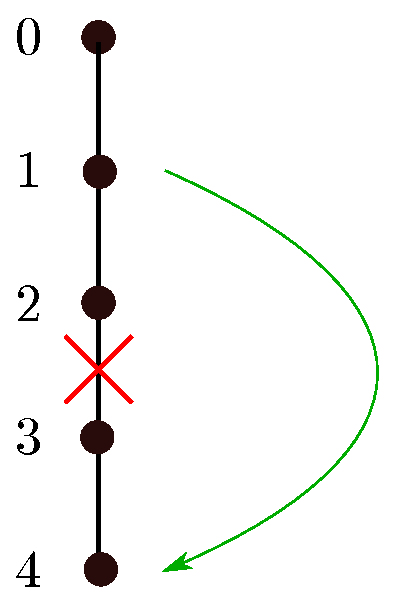
\includegraphics[width=0.2\textwidth]{pics/vertexExtensionRRT.eps}
   \caption{Schematic depiction of a initial polynomial solution with 4 segments. There is a collision in the third segment, marked as red cross. The replanning takes place between vertex 1 and vertex 4.}
   \label{pic:vertexExtensionRRT}
\end{figure}


\subsection{Threshold for the RRT* Replanning}\label{sec:RRTreplanning}

There has to be a user specified threshold which defines after how many vertex extension a segment is considered a difficult segment. In this master thesis, the RRT* replanning is triggered after one unsuccessful vertex extensions.\newline

Since one cycle of vertex extension defines a new vertex in every segment which is in collision, it is not trivial to find the difficult segment in the initial solution.

\begin{figure}[H]
   \centering
   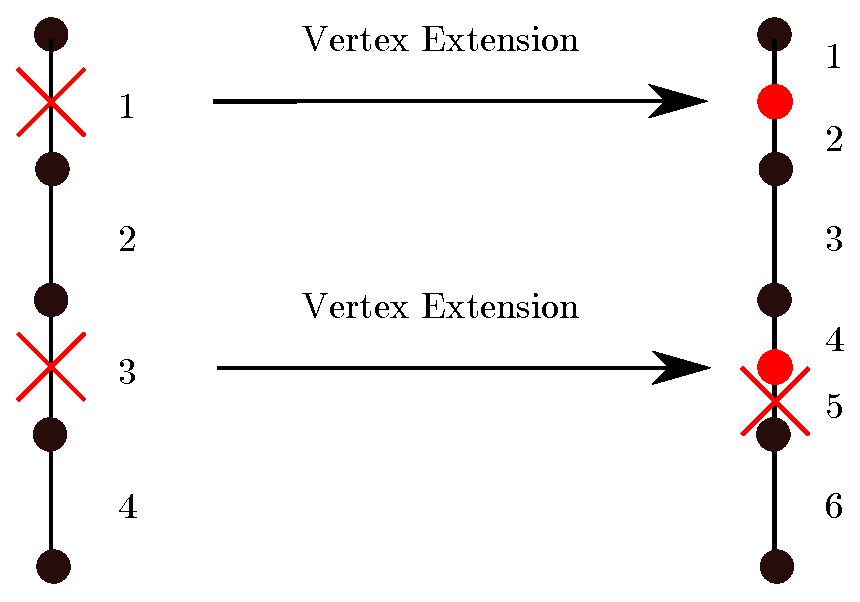
\includegraphics[width=0.6\textwidth]{pics/recogniseSegment.eps}
   \caption{One cycle of vertex extension. In the initial solution on the left-hand side of the figure there is a collision in segment 1 and segment 3. After one cycle of vertex extension there are 6 segments. }
   \label{pic:recognise}
\end{figure}

In figure \ref{pic:recognise} the segments are numbered. The left-hand side depicts the initial solution with a collision in segment 1 and segment 3. For both segments, a new vertex is added an illustrated as a red dot in the right-hand side of figure \ref{pic:recognise}. To find the difficult segment, 4 pairs of numbers have to be stored. The pairs consists of the initial segment which is in collision and of the corresponding segment after the vertex extension. \newline

The four pairs resulting from figure \ref{pic:recognise} are listed in the following table:

\begin{table}[H] 
\begin{center}
    \begin{tabular}{| c | c | c | }
    \hline
    Pair & Initial Segment & Extended Segment\\ \hline
   i) & 1 & 1 \\ \hline
   ii) & 1 & 2\\ \hline
   iii) & 3 & 4\\ \hline
   iv) & 3 & 5\\
    \hline
    \end{tabular}
    \caption{Four pairs of numbers, representing possible difficult segments. Every initial segment is connected to two extended segments.}
    \label{tab:pairsOfNumbers}
\end{center}
\end{table}

In the example depicted in figure \ref{pic:recognise} there is a collision in segment 5 after the vertex extension. 
Therefore, pair iv) gets significant and segment 3 (from the initial straight line solution) is exposed as a difficult segment.\newline

Once the difficult segment is located, the RRT* replanning can be performed as illustrated in figure \ref{pic:vertexExtensionRRT}.

\section{Overall Implementation}

All the features which are discussed so far can now be combined to the final implementation: \newline

\begin{figure}[H]
   \centering
   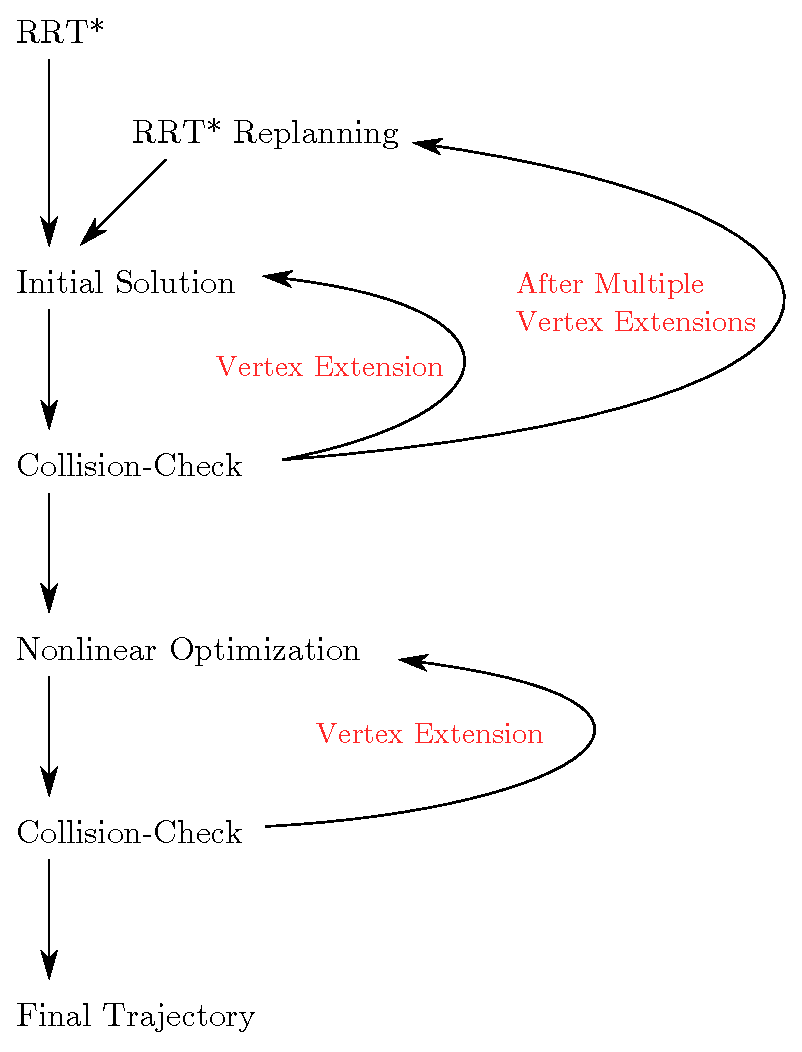
\includegraphics[width=0.6\textwidth]{pics/overall.eps}
   \caption{Schematic depiction of the final implementation of the path planning algorithm.}
   \label{pic:overall}
\end{figure}

Figure \ref{pic:overall} is simplified and does not describe all the necessary information but is useful to understand the basic process. For instance, the schematic depiction does not explain exactly how to proceed after the RRT* replanning and how many replannings should be allowed. 

\subsection{Store the Best Initial Solution}

As mentioned in section \ref{sec:RRTreplanning} the RRT* replanning is triggered after one unsuccessful vertex extensions. Caution, if a vertex extension is performed and this leads to a collision in a different part of the trajectory but the segment which was in collision in the initial solution is now collision free, no RRT* replanning is executed. \newline

A difficult segment in the initial solution does not mean that is impossible to find a collision free polynomial trajectory. Meaning the polynomial solution which is still in collision after one cycle of vertex extension, depicted in the right-hand side of figure \ref{pic:recognise}, can be collision-free after additional vertex extensions. If possible, the initial RRT* straight line solution is converted into a collision free polynomial trajectory with multiple vertex extensions and the polynomial trajectory and the corresponding total cost of the trajectory is stored. \newline

Not until then, the RRT* replanning is performed. The difficult section of the original straight line solution is then replaced by the replanned section and a polynomial trajectory passing trough the vertices is computed. The new trajectory on his part can be in collision and vertex extensions have to be performed until the trajectory is collision-free. Once the trajectory is collision-free, the total cost of the new trajectory is compared to the total cost of the first trajectory and the one with the lower cost is used for the nonlinear optimization.

\section{Robot Operating System}

The whole program is built using the \href{http://www.ros.org/}{Robot Operating System (ROS)} \cite{ROS}. To be exact, it is built as a ROS node. A node is a process that performs computation. Nodes are combined together into a graph and communicate with one another using streaming topics, services, and the Parameter Server. A very powerful feature of ROS is "Dynamic Reconfigure". This tool allows the user to change parameters during runtime. Runtime is the period of time when a program is running. It begins when a program is opened (or executed) and ends with the program is quit or closed.

\subsection{Dynamic Reconfigure}\label{sec:dynamicRec}

In this master thesis, several imported parameters are modifiable by Dynamic Reconfigure. Two of them mainly determine the performance of the RRT* algorithm:

\begin{itemize}
  \item $\gamma$
  \item $endRRT$
\end{itemize}

The $\gamma$ parameter determines the amount of rewiring and is described in detail in section \ref{sec:Rewiring}. $endRRT$ defines how many additional RRT* iteration are performed after a collision-free straight line connection is found. Thus, $endRRT = 2000$ leads to 2000 additional iterations in which the algorithm can improve the straight lines solution via rewiring. \newline

The next two parameters which are included into Dynamic Reconfigure are used to modify NLopt:

\begin{itemize}
  \item $J_{rel}$
  \item $k_T$
\end{itemize}


$J_{rel}$ is defined in section \ref{sec:NLopt} and is a ending criteria for NLopt. The weighting factor $k_T$ is defined in equation \ref{equ:total_cost} in section \ref{sec:penalty} and specifies the aggressiveness of a trajectory. \newline

The next parameter concerns the RRT* replanning. As explained in section \ref{sec:replanningPassages}, a RRT* replanning is beneficial if there are difficult passages in the initial straight line solution. It may happen, that the straight line solution with the replanned segments still has difficult passages. 

\begin{itemize}
  \item $maxReplanning$
\end{itemize}

$maxReplanning$ defines the max. number of RRT* replannings. After this number of replannings, the optimization starts with the best solution so fare. If no collision-free solution has been found, the complete RRT* planning starts again. \newline

The last parameter is bool parameter (either "true" or "false") affects the start vertex of a trajectory:

\begin{itemize}
  \item $currentPose$
\end{itemize}


$currentPose$ defines if the start vertex is either manually chosen or the actual current pose of the UAV. In this master thesis, the current pose is provided by \href{http://www.vicon.com/}{Vicon} \cite{Vicon}, a powerful object tracking solution providing unrivaled data accuracy for integration in to 3D applications. If $currentPose$ is set to "true" the current pose provided by Vicon is used as the start vertex.






%\subsection{Multiple Vertex Extension}

%\begin{figure}[h]
%   \centering
%   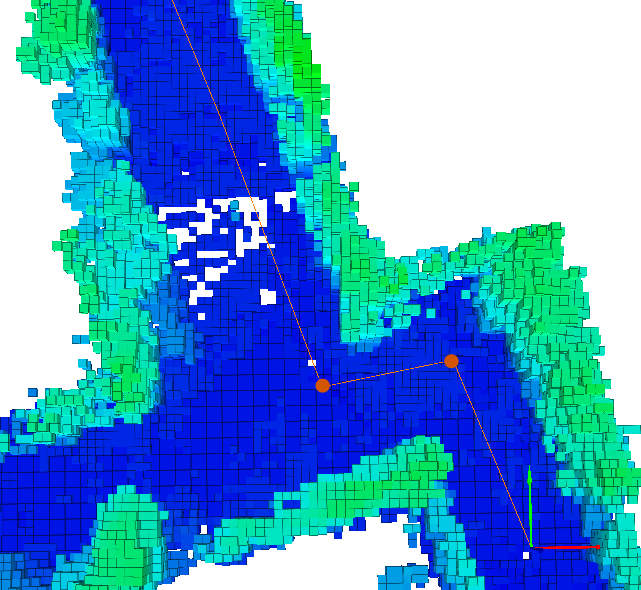
\includegraphics[width=1\textwidth]{pics/1LongP.png}
%   \caption{Ein Bild.}
%\end{figure}
%
%
%
%\begin{figure}[h]
%   \centering
%   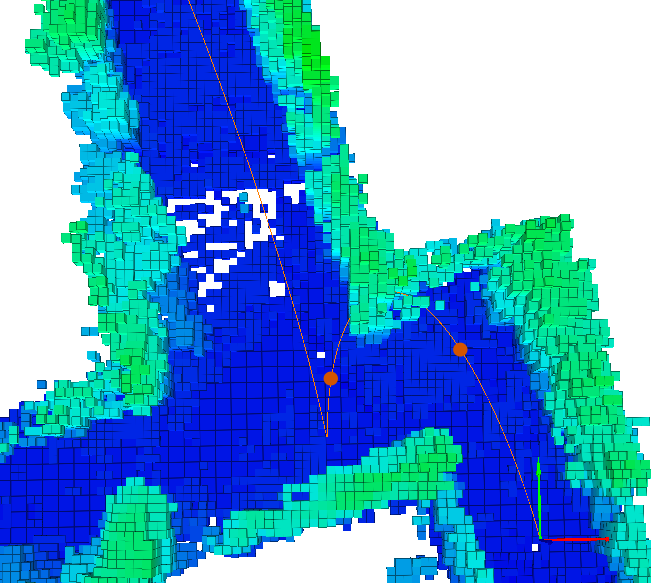
\includegraphics[width=1\textwidth]{pics/1aLongP.png}
%   \caption{Ein Bild.}
%\end{figure}
%
%
%\begin{figure}[h]
%   \centering
%   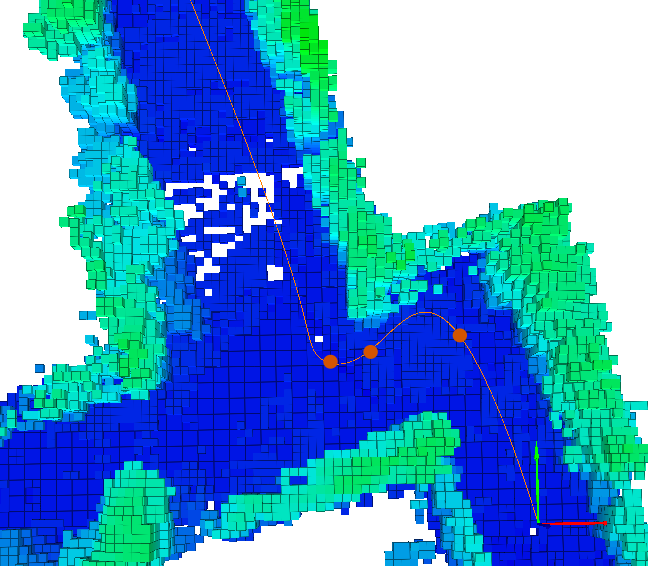
\includegraphics[width=1\textwidth]{pics/1bLongP.png}
%   \caption{Ein Bild.}
%\end{figure}
%
%\begin{figure}[h]
%   \centering
%   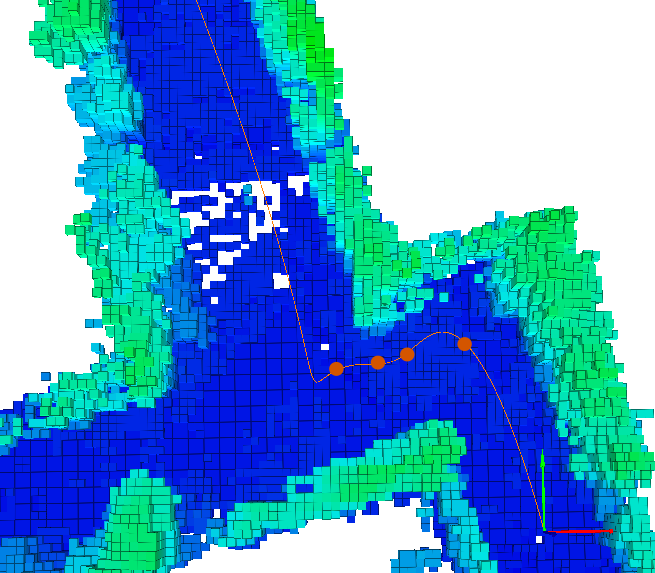
\includegraphics[width=1\textwidth]{pics/1cLongP.png}
%   \caption{Ein Bild.}
%\end{figure}
%
%\begin{figure}[h]
%   \centering
%   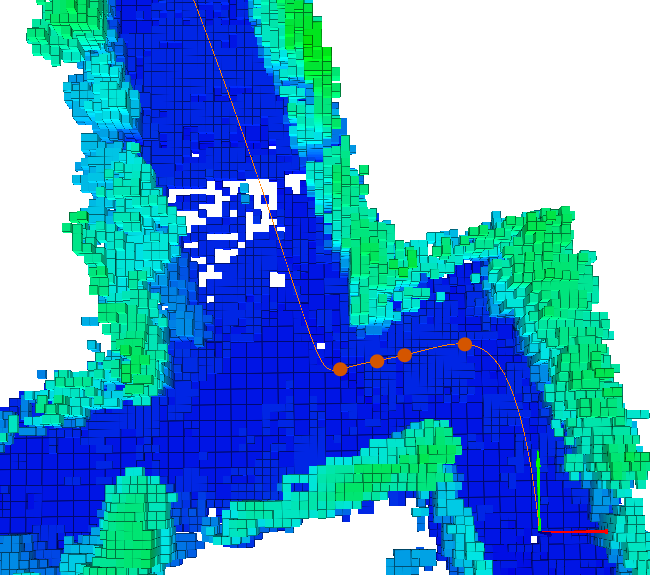
\includegraphics[width=1\textwidth]{pics/1dLongP.png}
%   \caption{Ein Bild.}
%\end{figure}
%
%

